\section[Les Internets et ses (dérives) d'usages]{Les internets et ses (dérives) d'usages}

\subsection{Les usages d'internets}

\begin{frame}{Concrètement, comment sont utilisés les internets ?}
  \begin{center}
    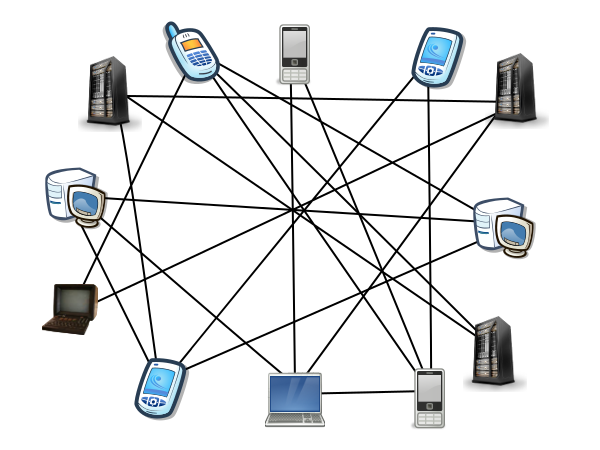
\includegraphics[height=0.8\textheight]{usages/reseau-bazar.png}
  \end{center}
\end{frame}

\begin{frame}{Concrètement, comment sont utilisés les internets ?}
  \begin{center}
    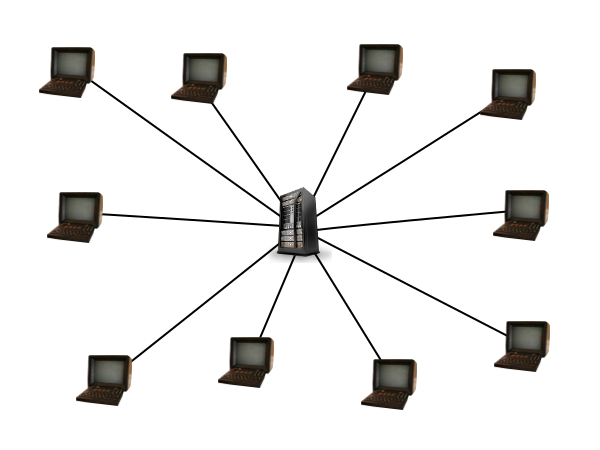
\includegraphics[height=0.8\textheight]{usages/reseau-etoile.png}
  \end{center}
\end{frame}

\subsection{Des dérives "économiques"}

\begin{frame}{Des dérives "économiques"\hfill(1/3)}
  \begin{center}
    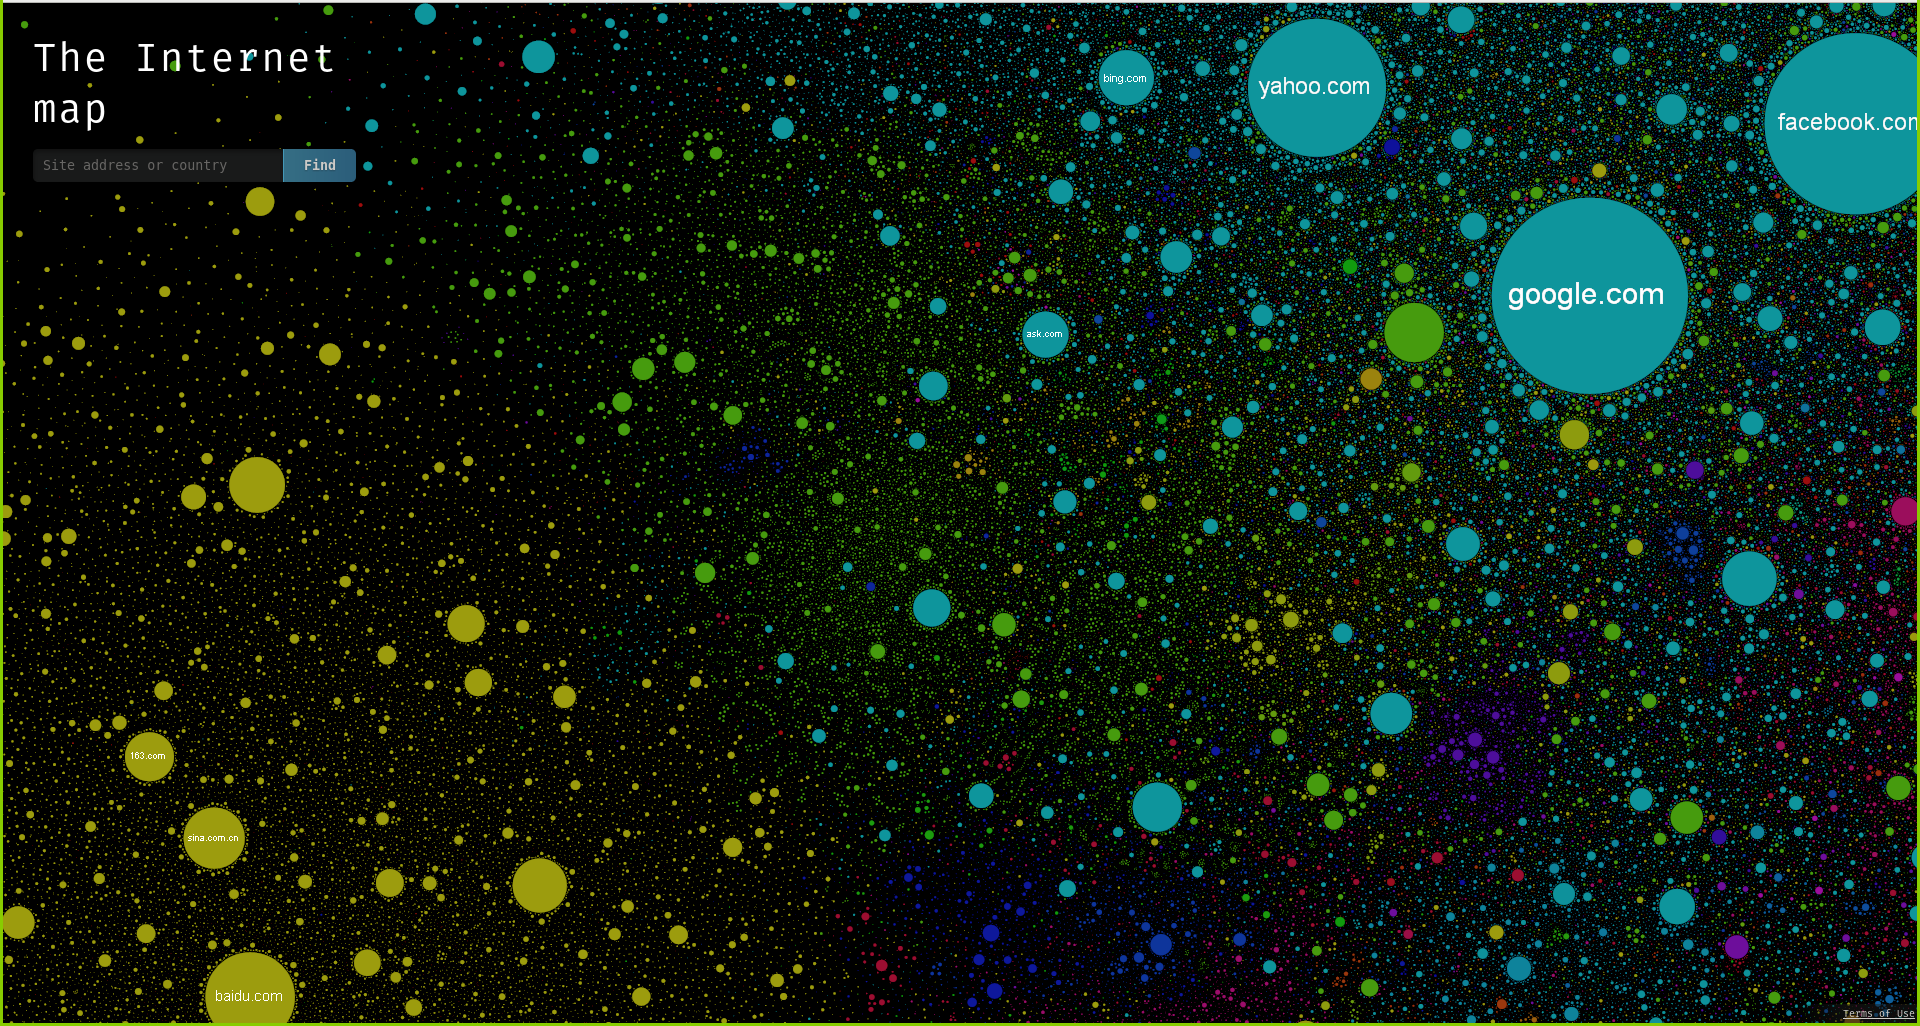
\includegraphics[width=1\textwidth]{usages/internet-map2.png}
  \end{center}
  \footnotesize{\tiny{source: https://internet-map.net}}
\end{frame}

\begin{frame}{Des dérives "économiques"\hfill(2/3)}
  \begin{center}
    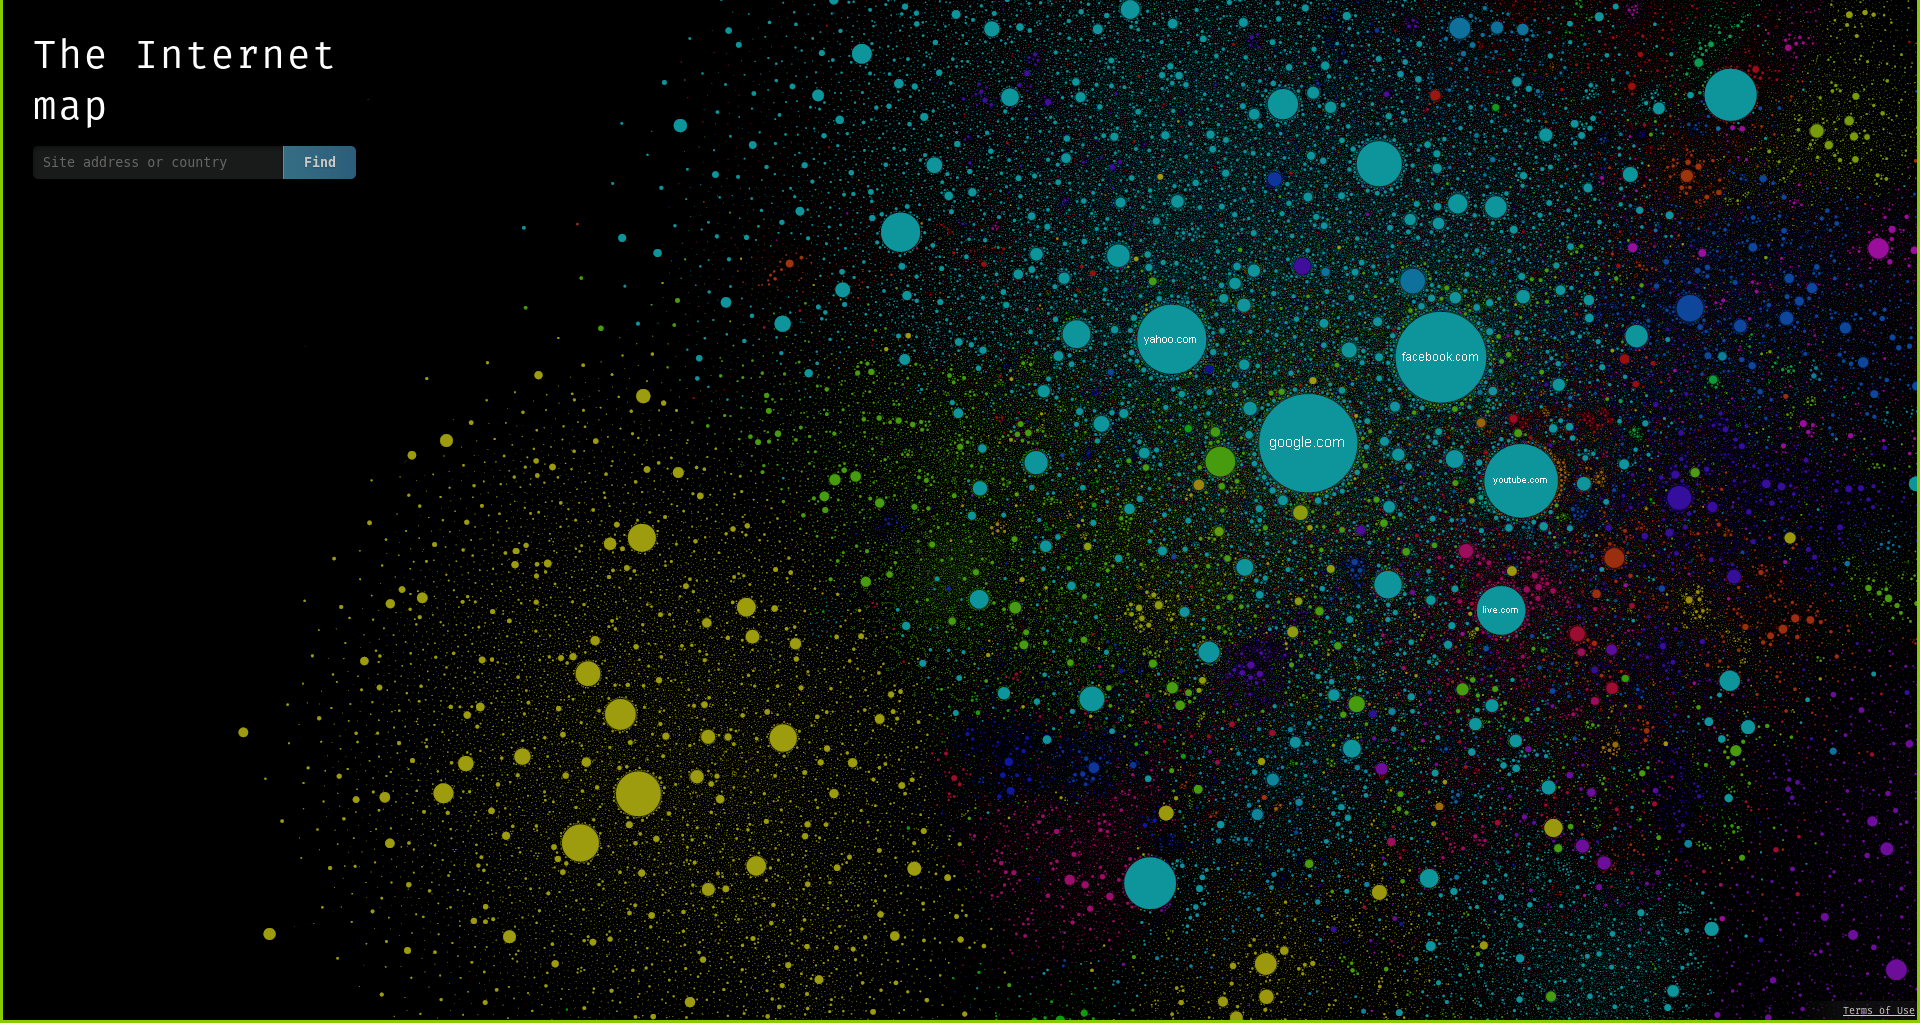
\includegraphics[width=1\textwidth]{usages/internet-map1.png}
  \end{center}
  \footnotesize{\tiny{source: https://internet-map.net}}
\end{frame}

\begin{frame}{Des dérives "économiques"\hfill(3/3)}
  \begin{center}
    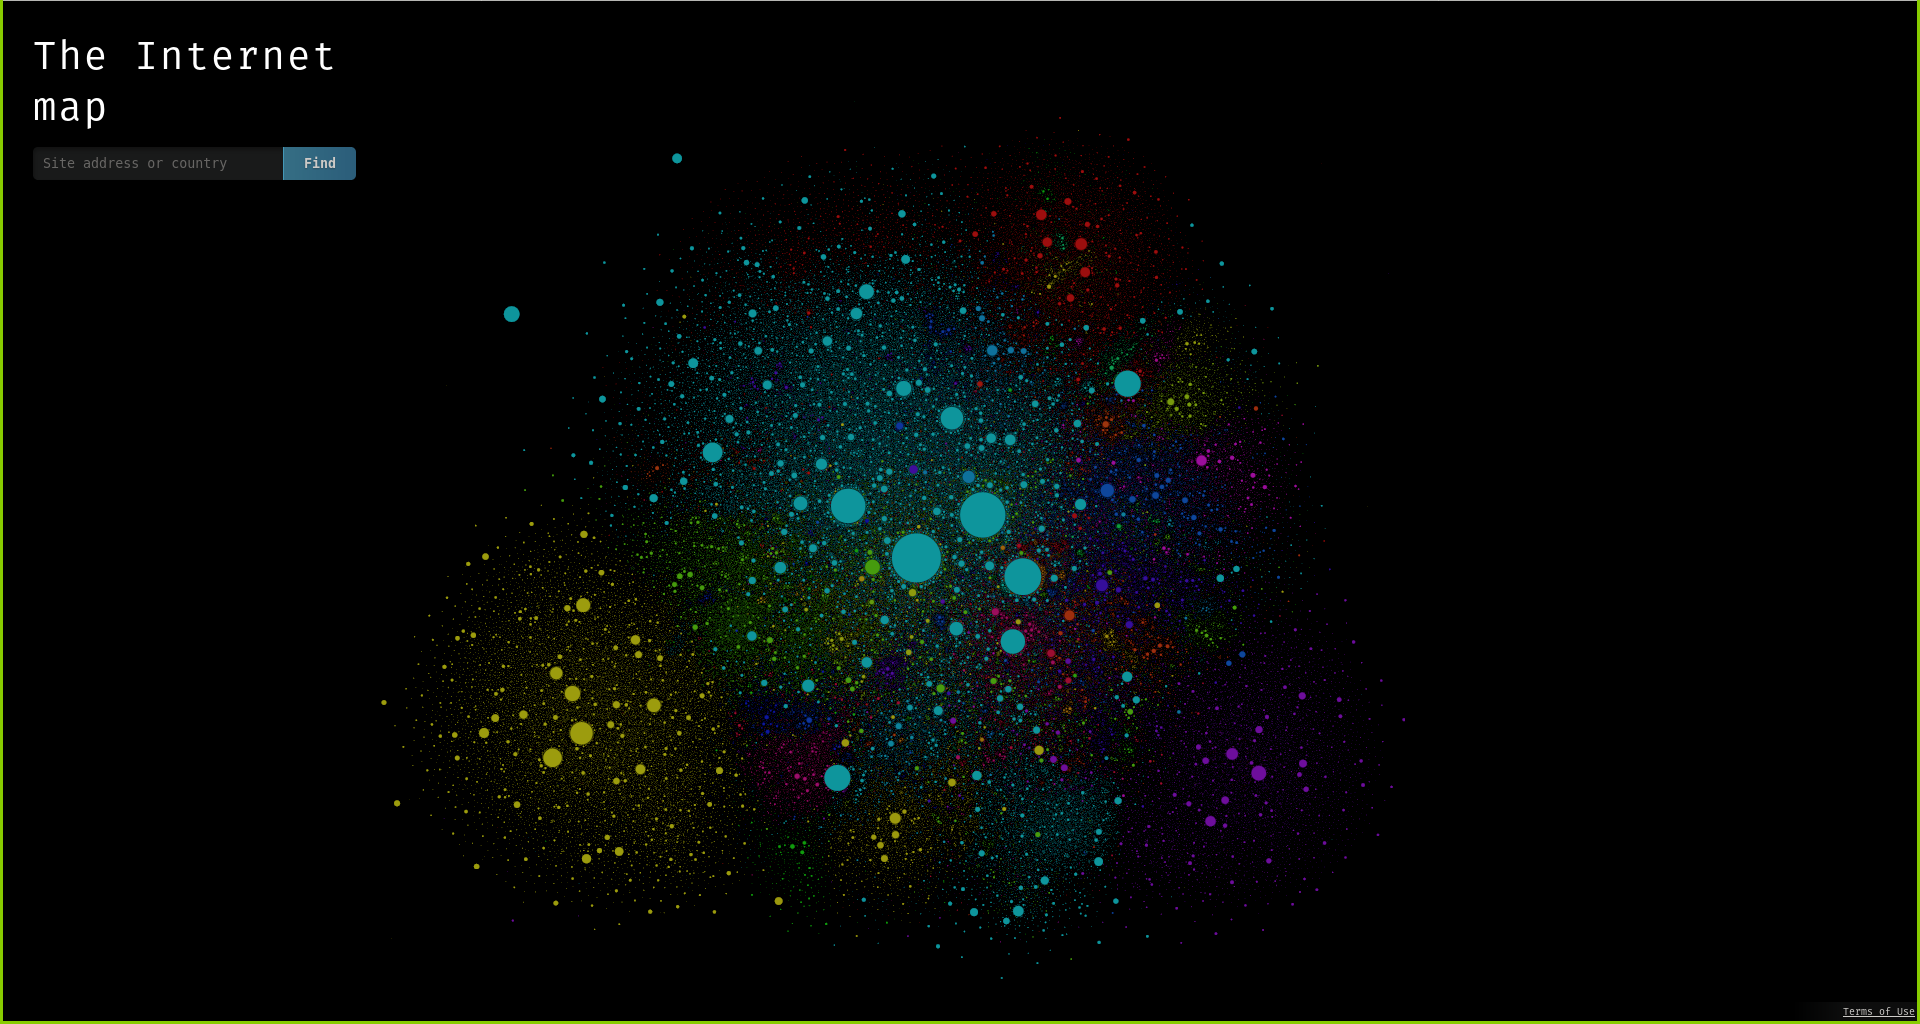
\includegraphics[width=1\textwidth]{usages/internet-map3.png}
  \end{center}
  \footnotesize{\tiny{source: https://internet-map.net}}
\end{frame}

\begin{frame}{Et ce n'est pas QUE la fautes des utilisateurs}
  \begin{columns}
  \begin{column}{0.5\textwidth}
    \raggedright\small
    Les interfaces graphiques:

    \begin{itemize}
      \item Le défilement "infini",
      \item La construction des pages,
      \item La lecture automatique de la vidéo suivante
      \item Et d'autre mécanismes...
    \end{itemize}

    Etudiées et choisies par des humains.
  \end{column}
  \begin{column}{0.5\textwidth}
    \begin{tikzpicture}
      \node (img1) {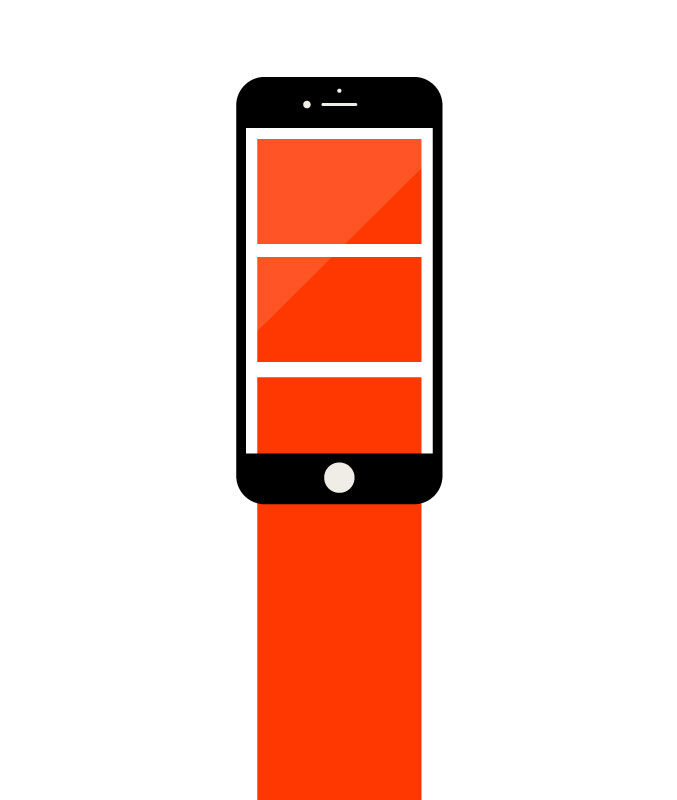
\includegraphics[width=.75\textwidth]{usages/scrolling.jpg}};
      \node (img2) at (img1.south east) {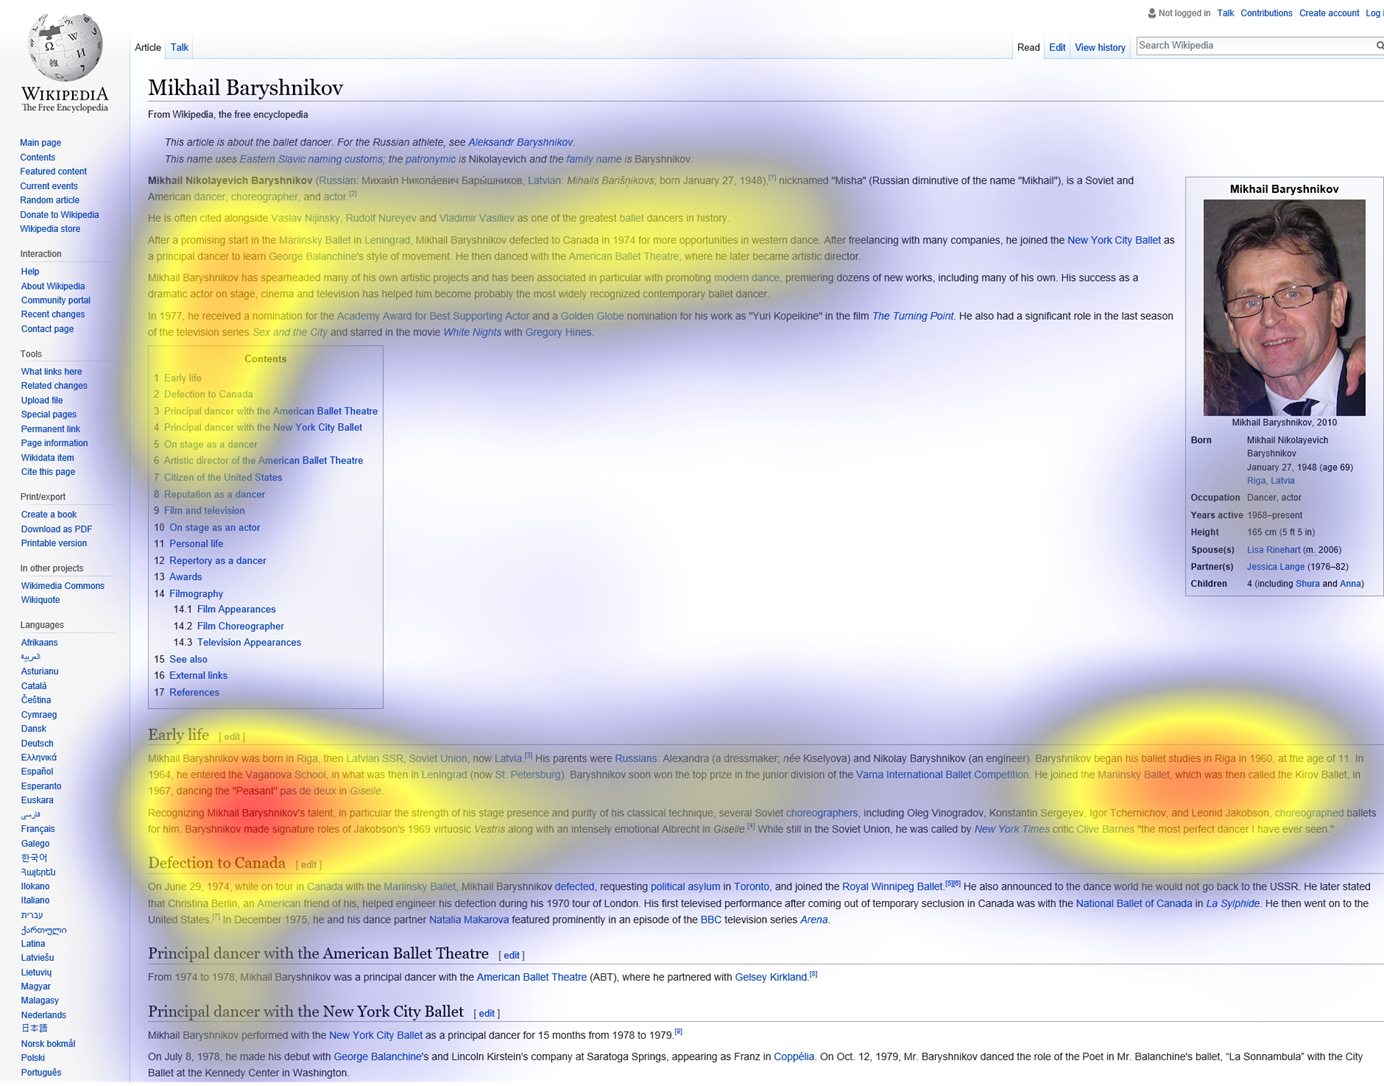
\includegraphics[width=.75\textwidth]{usages/f-pattern.png}};
    \end{tikzpicture}
  \end{column}
  \end{columns}
  \footnotesize{\tiny{source: https://mackeycreativelab.com/about-us/}}\\
  \footnotesize{\tiny{source: https://www.nngroup.com/articles/text-scanning-patterns-eyetracking/}}
\end{frame}


\begin{frame}{"L'intelligence artificielle" et les algorithmes}
    \small
    L'intelligence artificielle n'a rien "d'intelligent" ! \\
    Un algorithme ne décrit qu'une manière de faire, pas comment c'est fait \\
    {\centering
    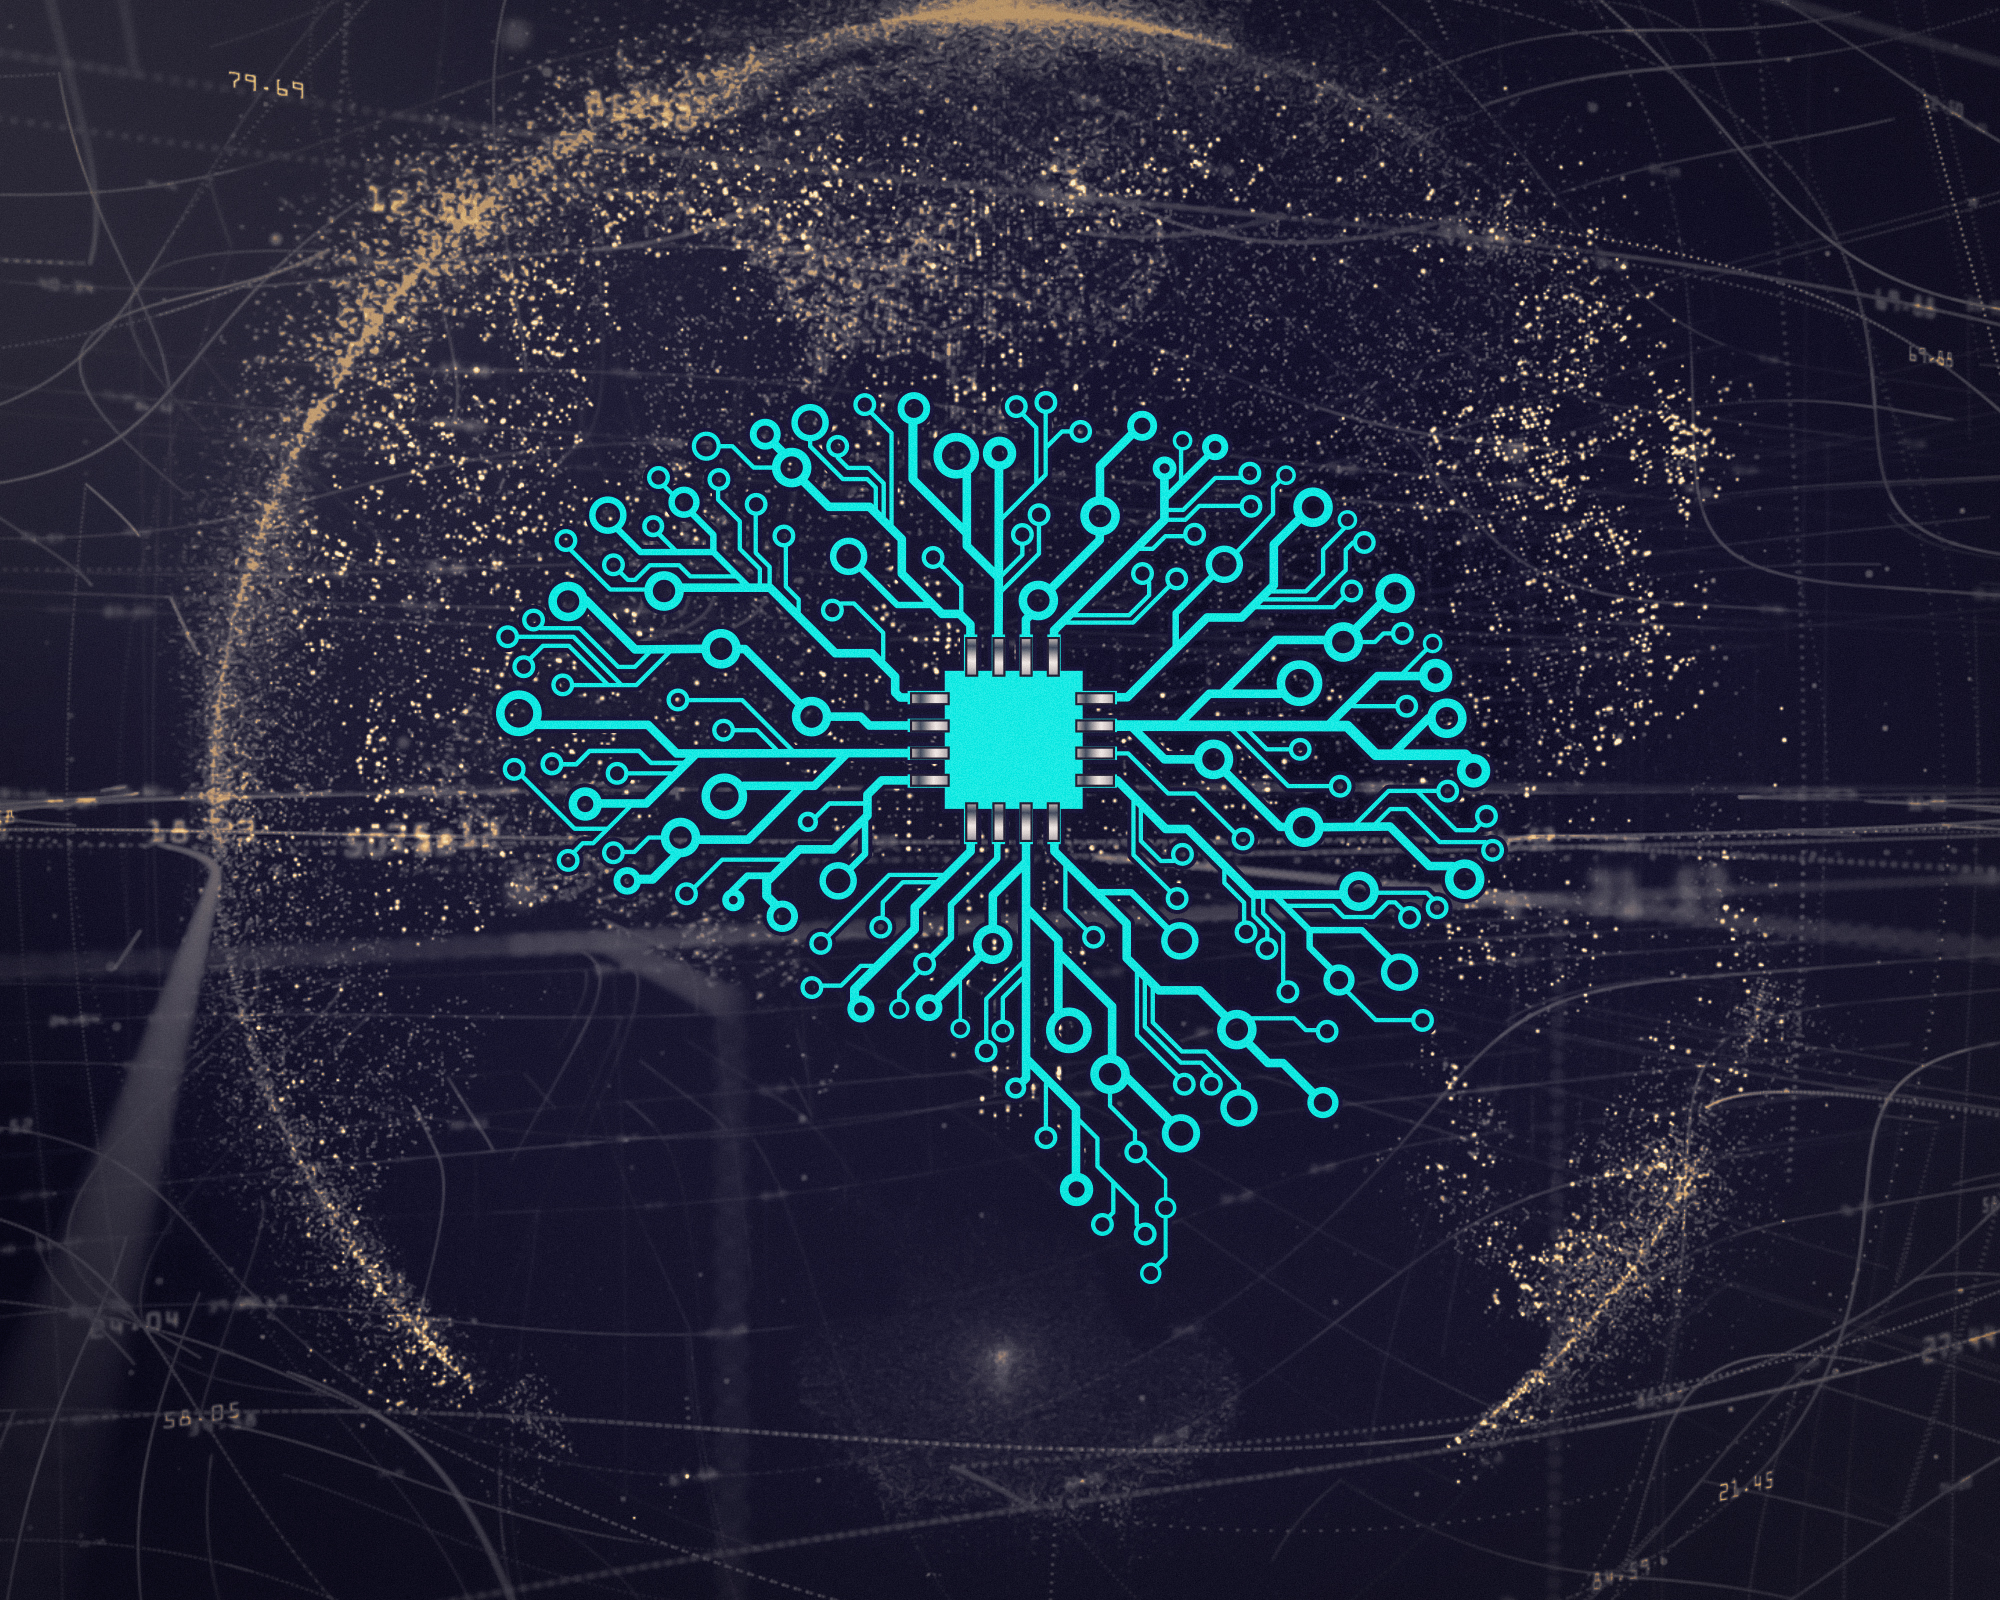
\includegraphics[height=0.7\textheight]{usages/intelligence-artificiel.png}\\
    }
  \footnotesize{\tiny{source: https://upload.wikimedia.org/wikipedia/commons/e/ee/Artificial\_Neural\_Network\_with\_Chip.jpg}}
\end{frame}

\begin{frame}{Oui, bon, les GAFAMs, tout ça...}
    \centering
    
\includegraphics[width=0.7\textwidth]{usages/gafam.png}
\end{frame}


\subsection{Des dérives plus "politique"}
\begin{frame}{\hfill ...mais pas que}
  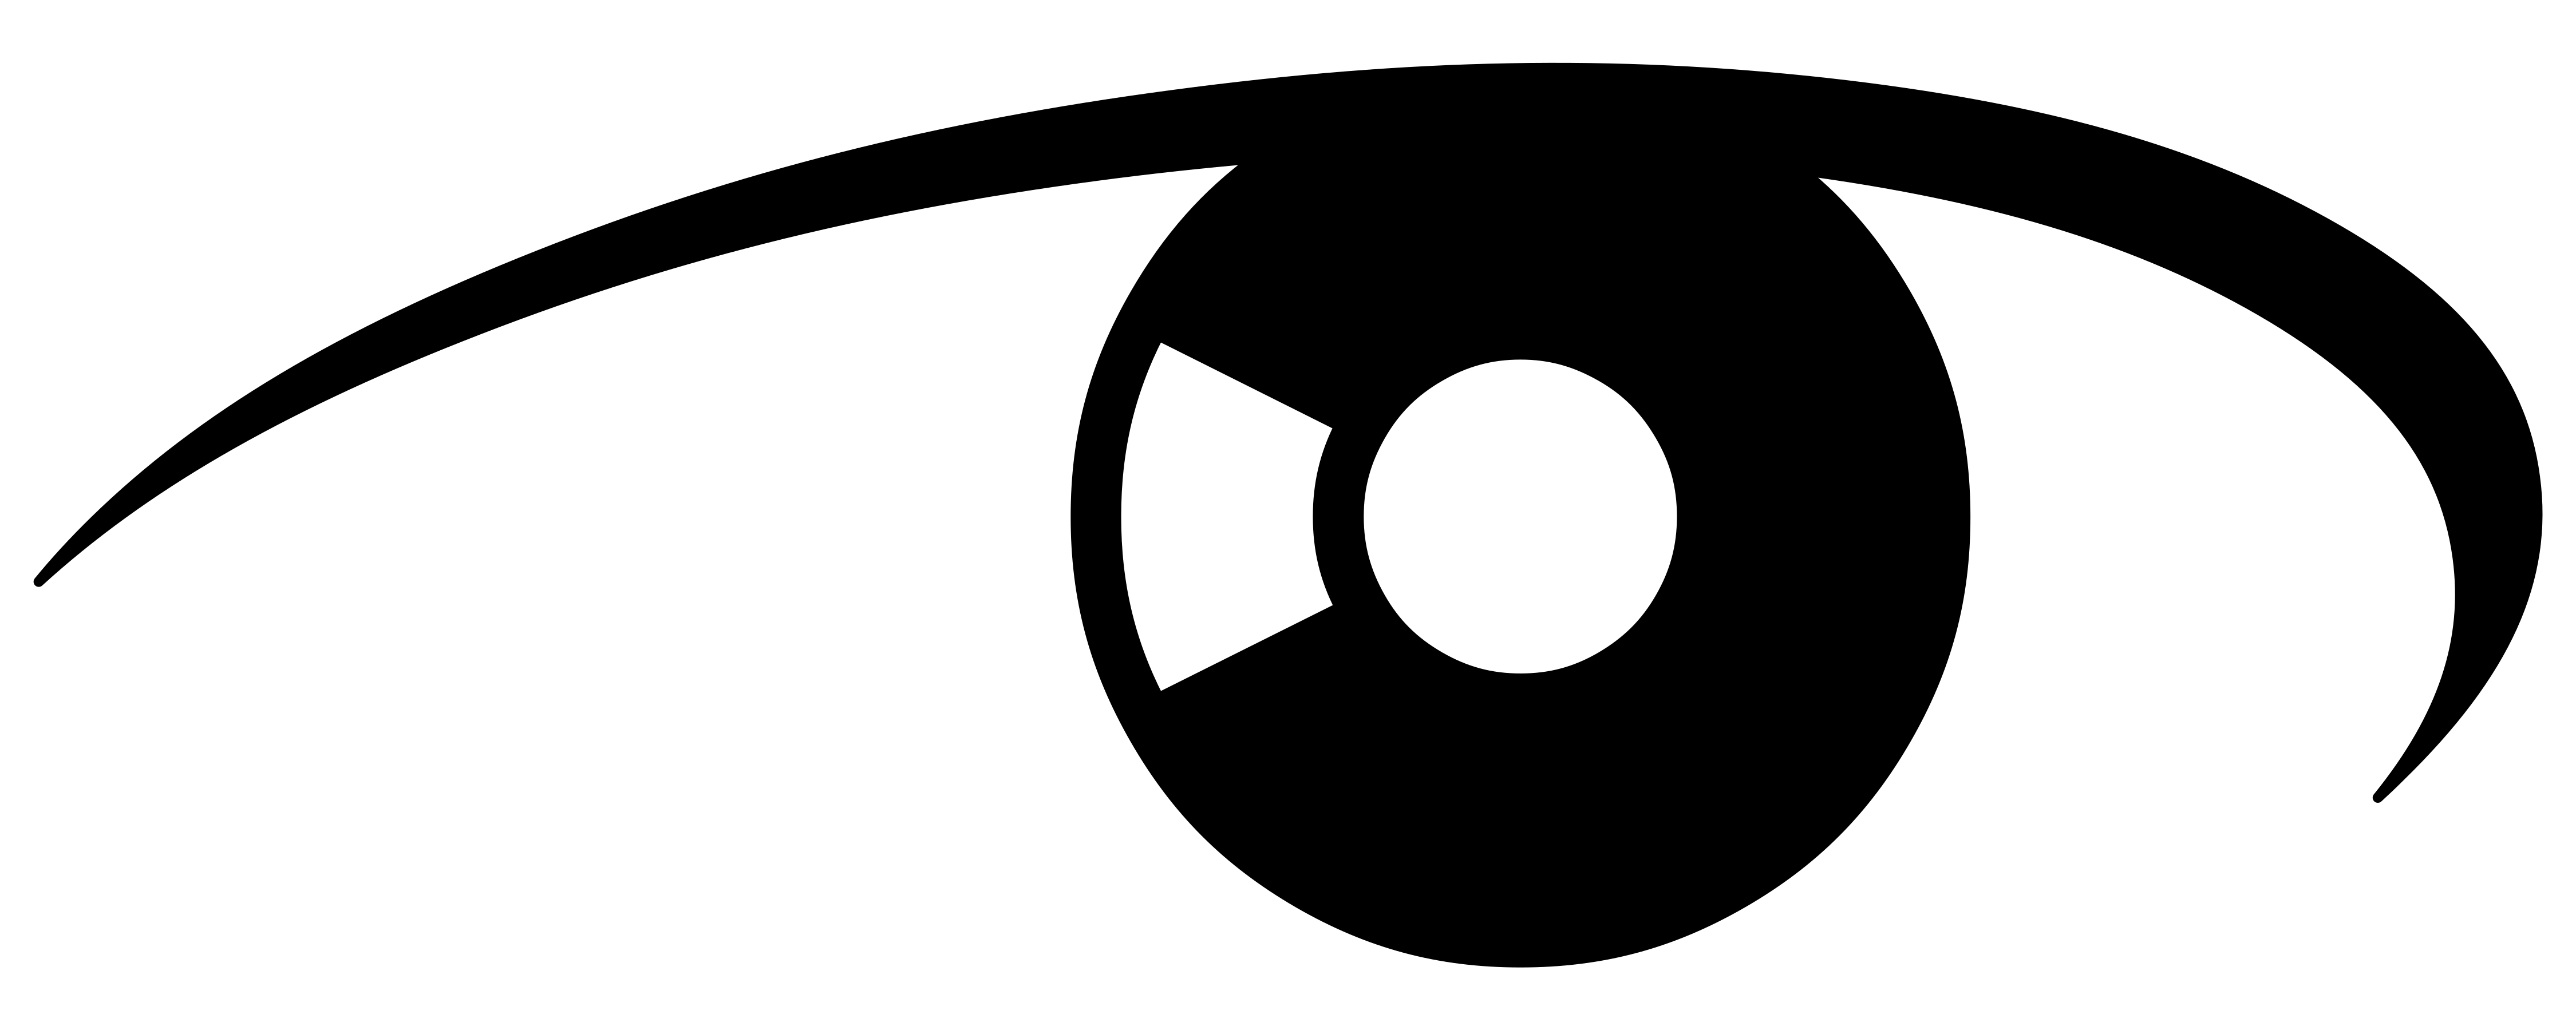
\includegraphics[width=\textwidth]{usages/oeil.png}
\end{frame}

\begin{frame}{La surveillance des espaces publiques}

  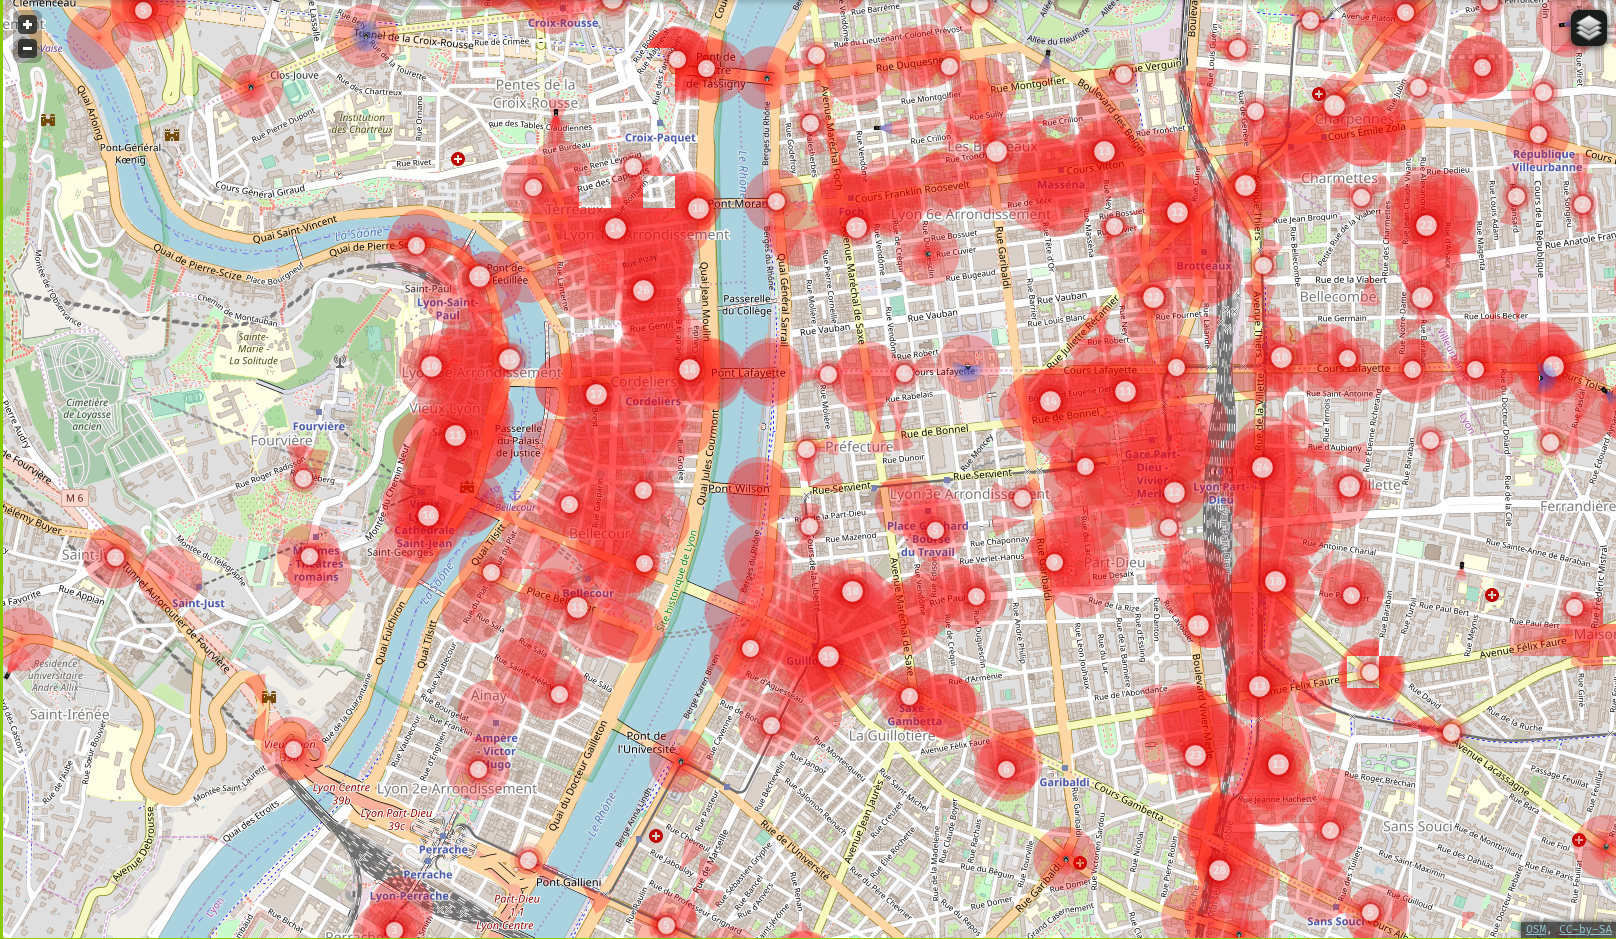
\includegraphics[width=\textwidth]{usages/surveillance_lyon.png}

  Décisions prises par des humains.

  \footnotesize{\tiny{source: https://lyon.sous-surveillance.net/}}
\end{frame}

\begin{frame}{La reconnaissance faciale}
  \tiny
  Expérimentation à Nice et Marseille

  30 Janvier 2020: \\
    - Abandon de l'UE pour l'interdire dans l'espace publique.

  \begin{center}
  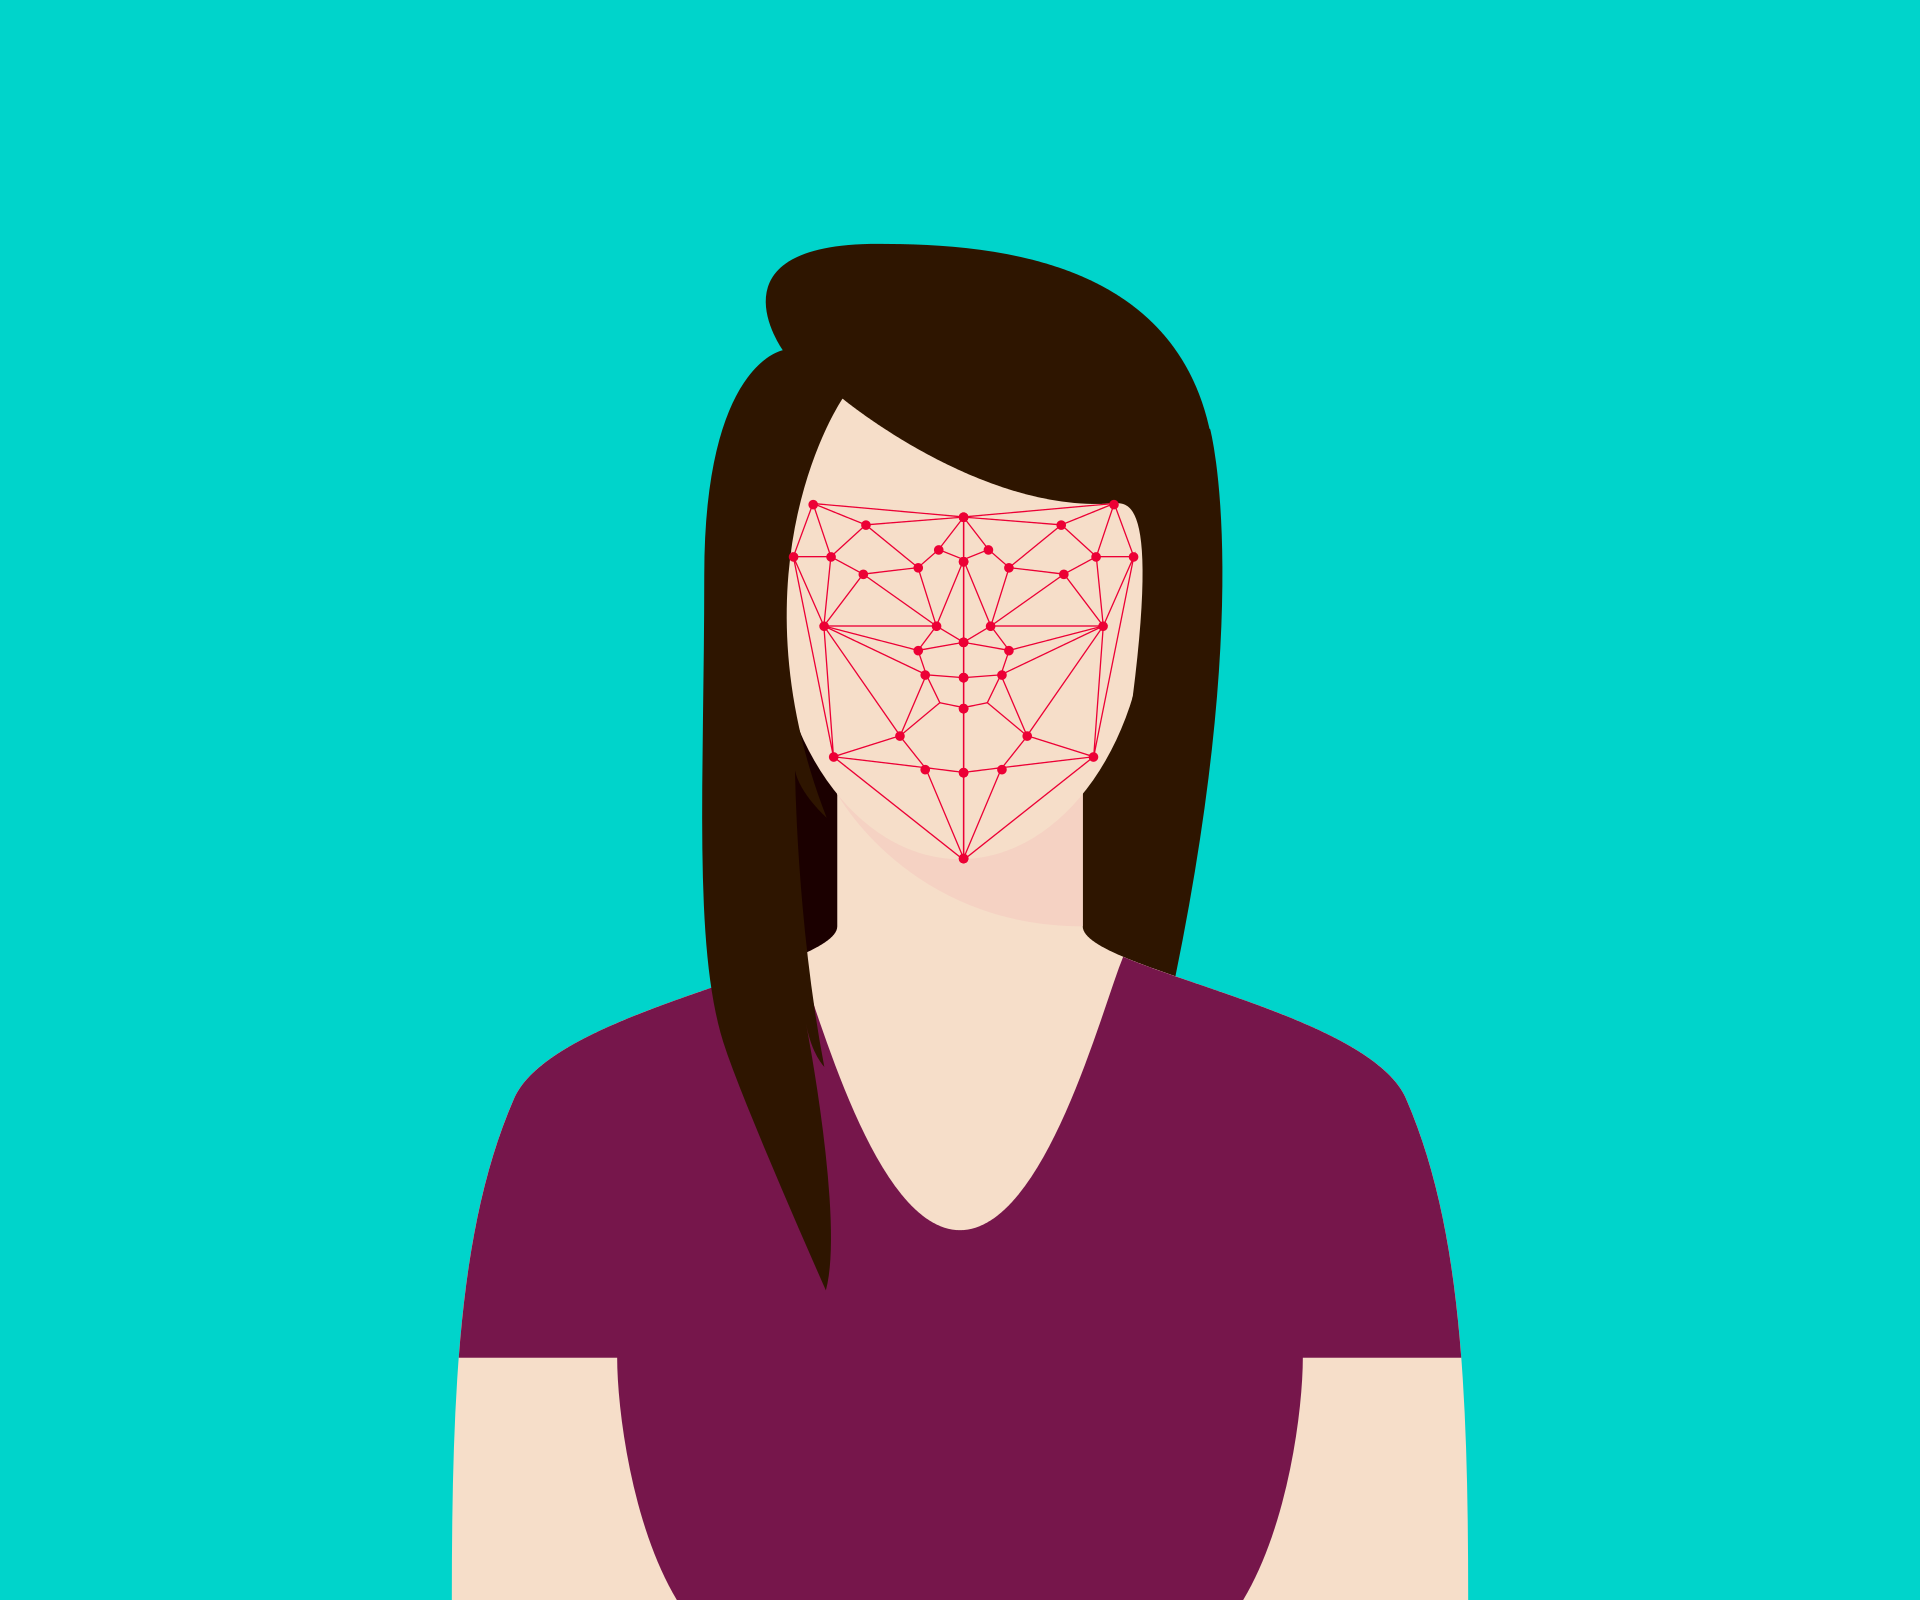
\includegraphics[width=.7\textwidth]{usages/reconnaissance_facial.png}
  \end{center}

  Décisions aussi prises par des humains.
\end{frame}

\begin{frame}{Fiscalité et médias sociaux}
  \small
  Autorisation du FISC français à utiliser les médias sociaux.

  \begin{center}
  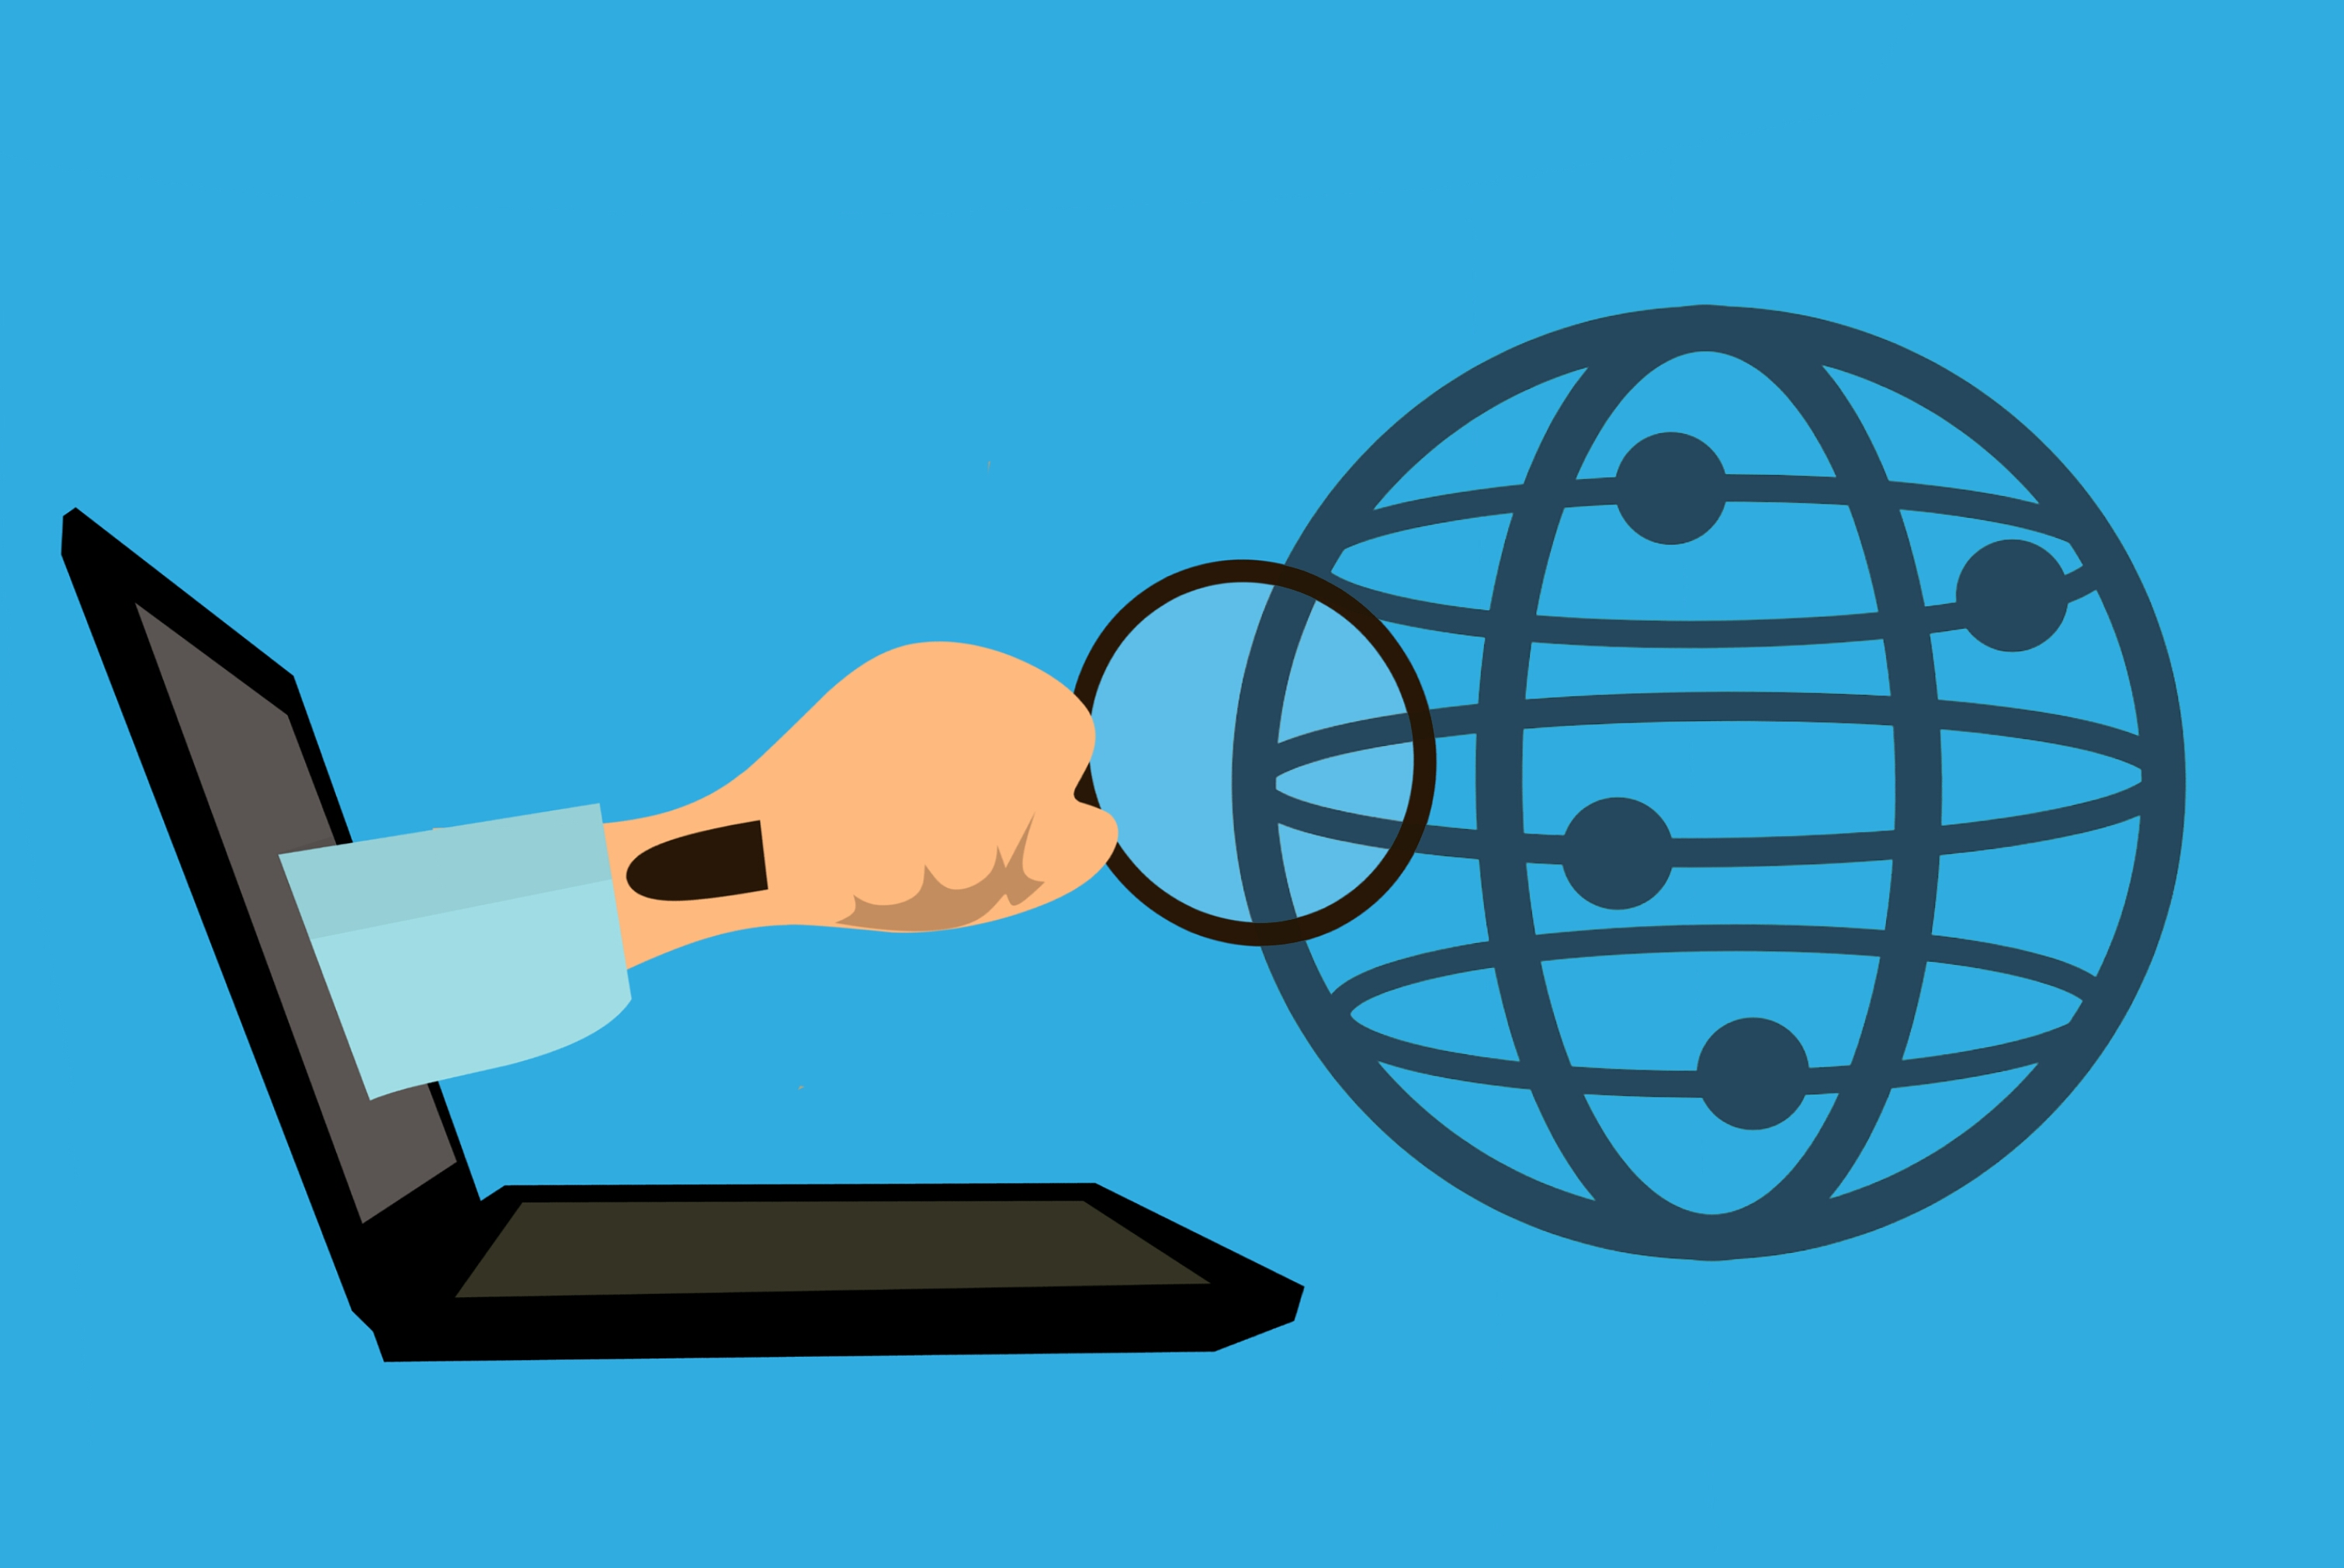
\includegraphics[width=.7\textwidth]{usages/loupe.jpg}
  \end{center}
\end{frame}

\begin{frame}{Système de "Crédit Social"}
  Expérimentation d'un système de réputation des citoyens en chine

  \begin{center}
  
\includegraphics[width=.7\textwidth]{usages/score.jpg}
  \end{center}
\end{frame}

\begin{frame}{Mais et les chats dans tous ça ?}
  \small
  Les internets, ce n'est pas que des machines.\\
  C'est surtout ce que les humains décident d'en faire, à tout les niveaux. \\

  Heureusement, nous pouvons essayer de faire autrement.

  \begin{center}
  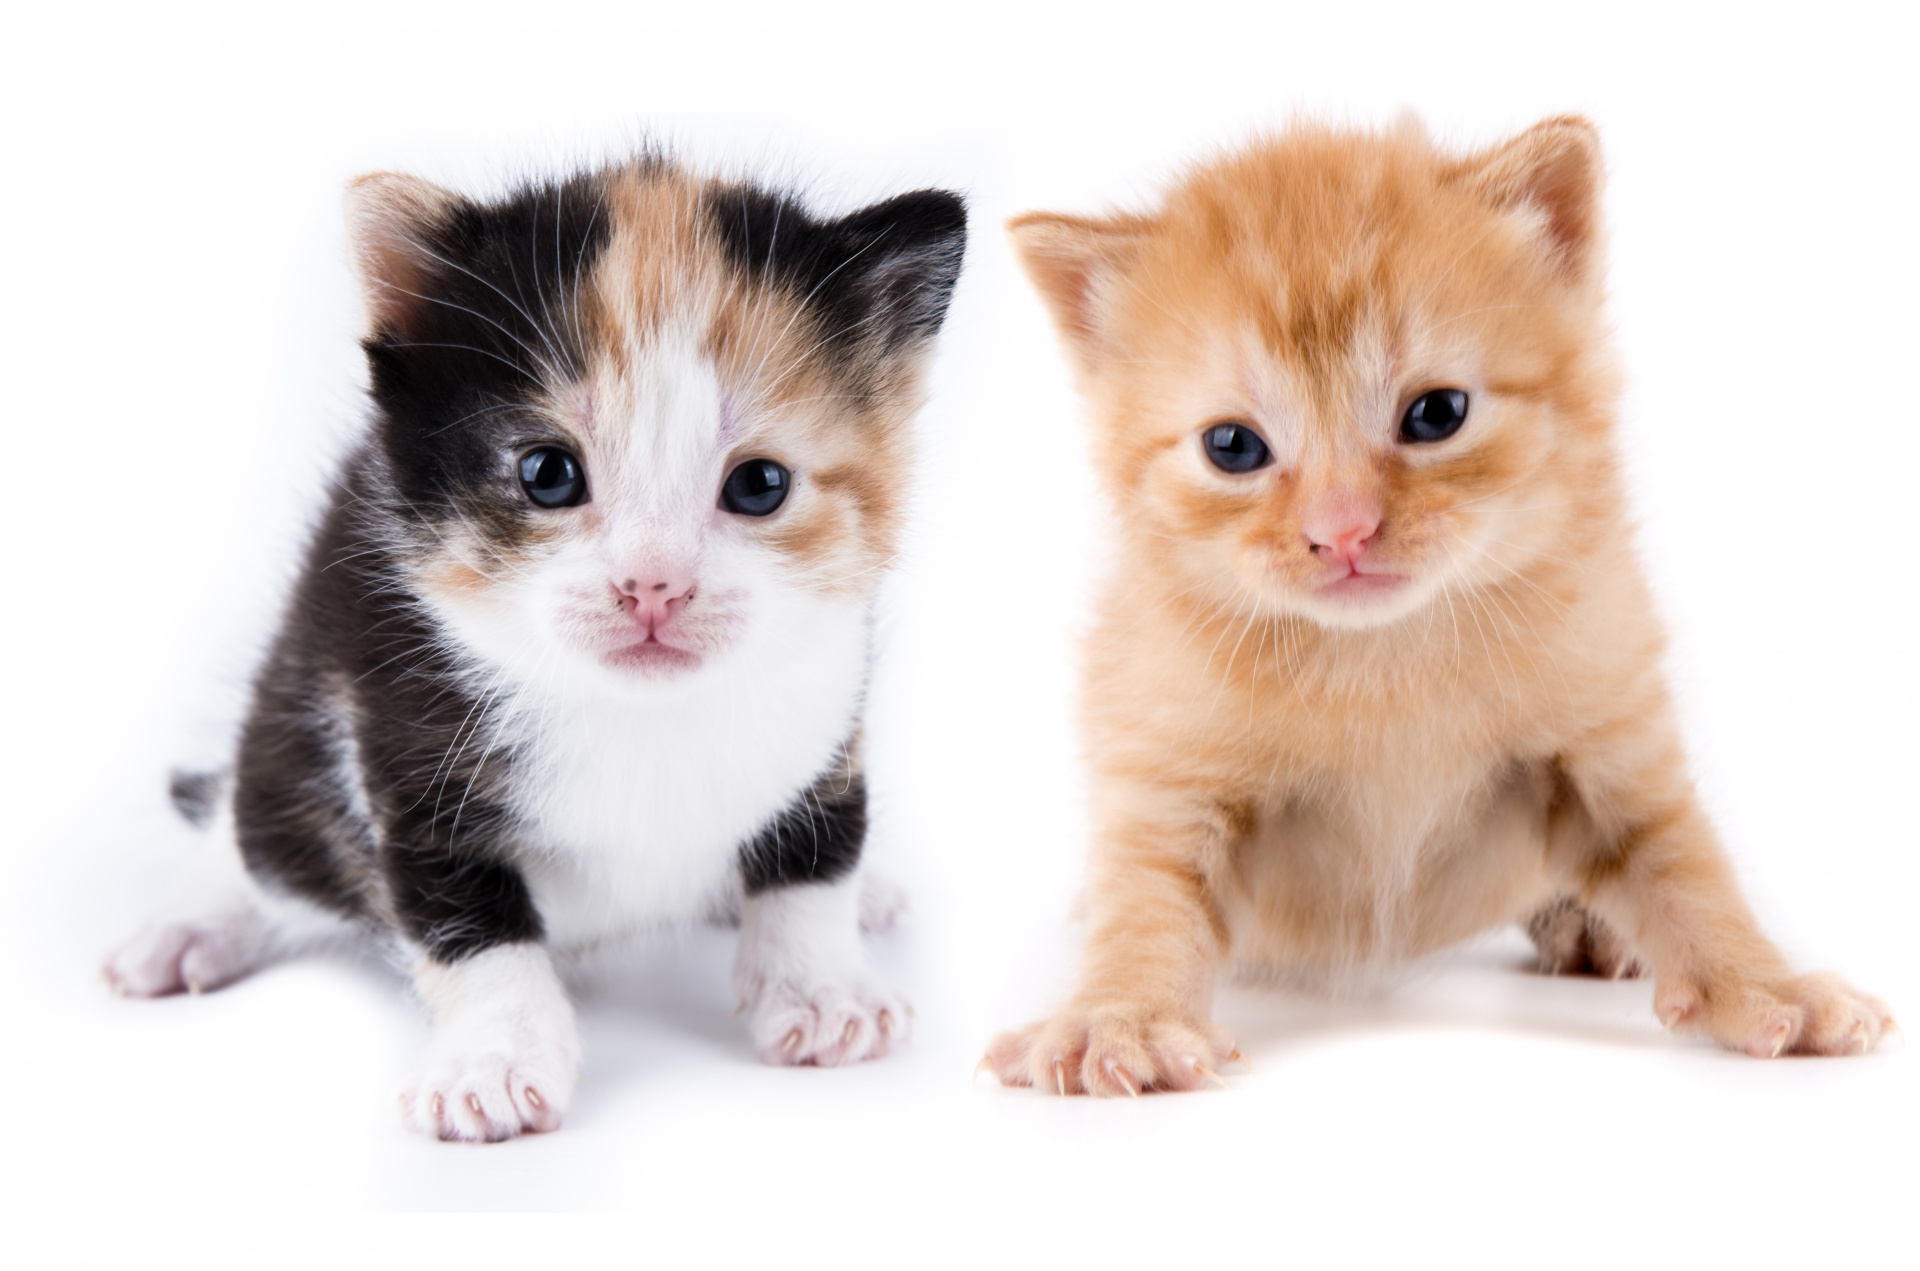
\includegraphics[width=.7\textwidth]{usages/chatons.jpg}
  \end{center}
\end{frame}

% vim: ts=2: sw=2: sts=2




